% This is "sig-alternate.tex" V2.1 April 2013
% This file should be compiled with V2.5 of "sig-alternate.cls" May 2012
%
% This example file demonstrates the use of the 'sig-alternate.cls'
% V2.5 LaTeX2e document class file. It is for those submitting
% articles to ACM Conference Proceedings WHO DO NOT WISH TO
% STRICTLY ADHERE TO THE SIGS (PUBS-BOARD-ENDORSED) STYLE.
% The 'sig-alternate.cls' file will produce a similar-looking,
% albeit, 'tighter' paper resulting in, invariably, fewer pages.
%
% ----------------------------------------------------------------------------------------------------------------
% This .tex file (and associated .cls V2.5) produces:
%       1) The Permission Statement
%       2) The Conference (location) Info information
%       3) The Copyright Line with ACM data
%       4) NO page numbers
%
% as against the acm_proc_article-sp.cls file which
% DOES NOT produce 1) thru' 3) above.
%
% Using 'sig-alternate.cls' you have control, however, from within
% the source .tex file, over both the CopyrightYear
% (defaulted to 200X) and the ACM Copyright Data
% (defaulted to X-XXXXX-XX-X/XX/XX).
% e.g.
% \CopyrightYear{2007} will cause 2007 to appear in the copyright line.
% \crdata{0-12345-67-8/90/12} will cause 0-12345-67-8/90/12 to appear in the copyright line.
%
% ---------------------------------------------------------------------------------------------------------------
% This .tex source is an example which *does* use
% the .bib file (from which the .bbl file % is produced).
% REMEMBER HOWEVER: After having produced the .bbl file,
% and prior to final submission, you *NEED* to 'insert'
% your .bbl file into your source .tex file so as to provide
% ONE 'self-contained' source file.
%
% ================= IF YOU HAVE QUESTIONS =======================
% Questions regarding the SIGS styles, SIGS policies and
% procedures, Conferences etc. should be sent to
% Adrienne Griscti (griscti@acm.org)
%
% Technical questions _only_ to
% Gerald Murray (murray@hq.acm.org)
% ===============================================================
%
% For tracking purposes - this is V2.0 - May 2012

\documentclass{sig-alternate-05-2015}

%%%%%%%%%%%% DEFINE PACKAGES HERE!!
\usepackage{algorithmic}
\usepackage{algorithm}
\usepackage{graphicx}
\usepackage{wrapfig}
%\usepackage{algpseudocode}
%\usepackage{minted}

\begin{document}

% Copyright
%\setcopyright{acmcopyright}
%\setcopyright{acmlicensed}
\setcopyright{rightsretained}
%\setcopyright{usgov}
%\setcopyright{usgovmixed}
%\setcopyright{cagov}
%\setcopyright{cagovmixed}


% DOI
\doi{XX.XXX/XXX_X}

% ISBN
\isbn{X-XXXXX-XX-X/XX/XX}

%Conference
\conferenceinfo{Bio331}{Fall 2016, Reed College, Portland, OR}

%\acmPrice{\$15.00}

%
% --- Author Metadata here ---
%\conferenceinfo{WOODSTOCK}{'97 El Paso, Texas USA}
%\CopyrightYear{2007} % Allows default copyright year (20XX) to be over-ridden - IF NEED BE.
%\crdata{0-12345-67-8/90/01}  % Allows default copyright data (0-89791-88-6/97/05) to be over-ridden - IF NEED BE.
% --- End of Author Metadata ---

\title{Grouping Badger Social Networks}
\date{\today}
%
% You need the command \numberofauthors to handle the 'placement
% and alignment' of the authors beneath the title.
%
% For aesthetic reasons, we recommend 'three authors at a time'
% i.e. three 'name/affiliation blocks' be placed beneath the title.
%
% NOTE: You are NOT restricted in how many 'rows' of
% "name/affiliations" may appear. We just ask that you restrict
% the number of 'columns' to three.
%
% Because of the available 'opening page real-estate'
% we ask you to refrain from putting more than six authors
% (two rows with three columns) beneath the article title.
% More than six makes the first-page appear very cluttered indeed.
%
% Use the \alignauthor commands to handle the names
% and affiliations for an 'aesthetic maximum' of six authors.
% Add names, affiliations, addresses for
% the seventh etc. author(s) as the argument for the
% \additionalauthors command.
% These 'additional authors' will be output/set for you
% without further effort on your part as the last section in
% the body of your article BEFORE References or any Appendices.

\numberofauthors{1} %  in this sample file, there are a *total*
% of EIGHT authors. SIX appear on the 'first-page' (for formatting
% reasons) and the remaining two appear in the \additionalauthors section.
%
\author{
% You can go ahead and credit any number of authors here,
% e.g. one 'row of three' or two rows (consisting of one row of three
% and a second row of one, two or three).
%
% The command \alignauthor (no curly braces needed) should
% precede each author name, affiliation/snail-mail address and
% e-mail address. Additionally, tag each line of
% affiliation/address with \affaddr, and tag the
% e-mail address with \email.
%
% 1st. author
\alignauthor
Karl Menzel\\
       \affaddr{Biology Department, Reed College}\\
       \affaddr{Portland, Oregon}\\
       \email{menzelk.edu}\\\date{\today}
}

\maketitle

\begin{abstract}
This ACM-style template describes how to typeset pseudocode as well as write common mathematical symbols.  \textbf{Copy this project and start by modifying the title, author, etc.}  There are also very useful URLS on Moodle for more information.
\end{abstract}

\keywords{pseudocode, algorithms, math, LaTeX}

\section{modivation}
\indent Animals of some species tend to not be randomly distributed throughout space, instead animals tend to be group up into populations and sub populational groups including social groups. Understanding these social groups can be important for understanding things such as the distribution of disease within the population \cite{weber-2013}, the social interactions and relationships \cite{Ramos-Fernadez-2009}, and interpopulation interactions \cite{marth-2011}. Computational methods using graphs methods have proven to be useful when identifying and social groups and subgroups in highly dynamic free ranging systems \cite{Ramos-Fernandez-2009,marsh-2011}. These clustering studies have used weighted graphs created by some measure of association whether by observational studies or by radio collars. Weber et. al. (2013) does not implement clustering on their badger social network, but they use measures of flow-betweennes which are used on some clustering methods.  

\indent Most betweennes meausures just use some sort of shortest path method when calculating betweenness.  This can leave out some important information about other interactions where information can flow.  Information can flow along longer or more circuitous paths and so this should be accounted for in out measure of betweennes \cite{freeman-1991}.  Flow-betweenness does account for this, keeping track of all of the flow that can get between node when calculating betweenanes.
\begin{figure}{t}
%\centering % center the figure
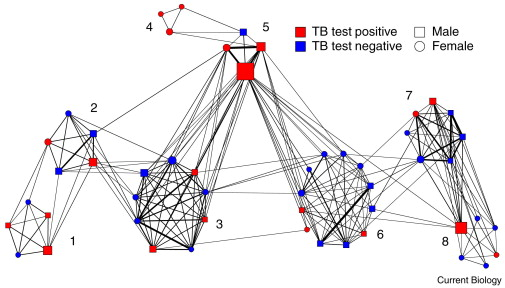
\includegraphics[width=\linewidth]{weberImage.jpg}
\caption{Figure form weber et. al. (2013) ilistrating the social interactions of badgers and distrobution of TB} % caption
\label{badger} % add a label to reference it
\end{figure}

\indent  Understanding the social groups of these badgers as well as understanding how flow-betweennes, within and between groups, plays into their social groups.


\section{Methods}

\subsection{data}

The data is an updated version of the data used in Weber et. al. (2013). This data was requested by Anna Ritz in the early fall of 2016.The data is held in two files BadgerInfo.txt and BadgerMatrix.txt.
\begin{itemize}
\item \textbf{BadgerInfo.txt} This contains demographic information about the badgers in in the study. It contains four columns: badger name, sex, whether or not they are infected with tuberculosis, and the social group the badger is a part of.

\item \textbf{BadgerMatrix.txt} This contains the interaction data of the badgers. This matrix is constructed as usual with each cell being the interaction between the row and column badger. The number in the cell denotes the amount of time that the two badgers were in close contact
\end{itemize}


\subsection{Pseudocode}
The goal is to find the flow-betweenness centrality of all of the nodes in the graph.  To do this I use alorgithm \ref{FBC} to get the normalized amount of flow calculated though each pair of points.  This algrorithm uses the Fodr-Fulkerson method to caluclate individual flows though nodes.  I seperate the flows into four different sections which use different subsets depending on which social group the node in question and to the sorce and target node are from.  First, $c_{total}$ inlcudes all of the possible pairing of source and sink nodes.  Seccond $c_{btwn}$ consists of sorce and target are not from the same socal group.  The next two are if the source and the target are in the same social group: $c_{inter}$ has the node in question in that same social group, $c_{out}$ has the node in question in a different social group. Algorithm \ref{FBC} interates between all unique combinations of sources and targes with $(u,v) = (v,u)$ and at each combination finds the normalized flow for all the nodes using \ref{FF}.  It then addes those flows to the centrality group that they are a part of.  


\begin{algorithm}[b]
\caption{Ford-Fulkerson method}
\label{FF}
\begin{algorithmic}
\STATE $\text{ \textbf{Inputs:} A network } G = (V, E) \text{ with flow capasity } c, \text{ source } s, \text{ and target } t$ 
\STATE $ \text{ \textbf{Outputs:} Flows } f(u, v) \text{ for all }(u, v) \in E \text{ between }s \text{ and }t$
\STATE $f(u, v) \leftarrow 0 \text{ for all edges } (u, v)$
\WHILE{  $\text{there exits a path } p \text{ in } G_{f} : c_{f} (u,v) > 0 \text{ for all edges } (u, v) \in p$}
\STATE find $c_{f}(p) = \min (c_{f}:(u, v) \in P)$
\FOR{each edge $(u,v) \in p$}
\STATE  $f(u, v) \leftarrow f(u,v) + c_{f}(p)$
\STATE  $f(v, u) \leftarrow f(v,u) - c_{f}(p)$
\ENDFOR
\ENDWHILE
\RETURN $\mathbf{f}$
\end{algorithmic}
\end{algorithm}


The Ford-Fulkerson method (Algorithm \ref{FF}) works by simulating putting flow throught the graph.  It does this by keeping track of a residual network ($G_{f}$) which is a representation of how much more flow can go through each of the edges.  The algorithm goes until there is not path from the source to the sink where all of the edges $>$ 0 in the residual graph.  In other words this is untill there can be no more flow to the target from the source.  Each iteration the algorithm find a path using depth first search on $G_{f}$, then it adds the minimun edge$ c_{f}$ value to each of the flows and the recalculates $G_{f}$.  This is like sending the most possible flow though that path which is restricted by edge with the lowest flow.  Once there are no more paths in $G_{f}$ from the source to the target it will return the flows for each of the edges in G.


\begin{algorithm}[t]
\caption{Flow-Betweenness Centrality}
\label{FBC}
\begin{algorithmic}
\STATE \textbf{Inputs:} $G(E,V)$ and edge weights $w$ social groups s
\STATE \textbf{Outputs:} flow-betweenness centrality for nodes
\STATE $c_{inter}(n) \leftarrow 0 \text{ for } n \in E$
\STATE $c_{btwn}(n) \leftarrow 0 \text{ for } n \in E$
\STATE $c_{out}(n) \leftarrow 0 \text{ for } n \in E$
\FOR {$k \in V$}
\FOR{$j \in V : (j,k) \in E \text{ and } j < k$}
\STATE $ f(u,v) = \text{Ford-Fulkerson} (G,w,j,k)$
\FOR{n $\in V : n \neq j \text{ and } n \neq k$}
\STATE $c(n) = \sum_{o \in N(n)}\frac{| f(n,o)|}{2 (\sum_{o \in N(k)}|f(k,o)|)} \text{ where } N(n) \text{ are n's neigbors} )$
\IF { $s(j) = s(k) \text{ \textbf{and} } s(j) = s(n)$}
\STATE $c_{inter}(n) = c_{inter}(n) + c(n)$
\ELSIF {$s(j) = s(k)$}
\STATE $c_{out}(n) = c_{out}(n) + c(n)$
\ELSE 
\STATE $c_{btwn}(n) = c_{btwn}(n) + c(n)$
\ENDIF
\STATE $c_{total}(n) = c_{total}(n) + c(n)$
\ENDFOR
\ENDFOR
\ENDFOR
\RETURN $c_{total}, c_{inter}, c_{btwn}, c_{out}$
\end{algorithmic}
\end{algorithm}




I also used the Girvan-Newman method to cluster the nodes based on both the edge flow betweenness and the raw edges weights.  The Girvan-Newman method works by finding the betweenness of each of the edges.  It does this by finding the shortest path between every pair of nodes and then find the number of these paths that each edge is in, then it removes the edge with the highest betweenness.  Then the betweennes of all the effected edges are recalculated and another edge is taken off.  To find a certain number of groups, those steps are repeated until there are the desired number of connected components.

\section{results}

\begin{table}[b]
\centering
\label{table}
\caption{Summary of whether edges that start in a social group end in the same social group or another social group.}
\begin{tabular}{| c | c | c  | }
\hline
Group & Num Group Edges &  Internal Edges (\%)\\
\hline
1 & 109 & 66 \\
\hline
3 & 44 & 55 \\
\hline
2 & 9 & 67 \\
\hline
5 & 60 & 20 \\
\hline
4 & 41 & 49 \\
\hline
7 & 76 & 53 \\
\hline
6 & 27 & 74\\
\hline
8 & 128 & 72\\
\hline
\end{tabular}
\end{table}

This data consists of all of the interactions of 52 badgers. This population of badgers consists of 9 social groups which are defined by the setts (tunnel system) where they live. Following are statistics that represent the proportion of these interaction that are between members of the same social group and between members that are not in the same social group as well as aggregates for each social group. In table \ref{table} Number of Edges on Nodes in Group is found by $|(i,j) : (i,j) \in E$ and $ i \in S_i| $ given nodes i and j in graph G = (V,E) and social group $s_i$ and the next column is the proportion of those edges that had one edge outside the social group.

\indent Figure \ref{bace} visualizes the full badger network with my calculated variables.  The node sizes are a scaled version of node between group flow betweeness.  The edge thicknesses represent the edge flow-betweenness. The badger network was clustered by the Girvan-Newman method using both the raw time data and the edge flow betweenness as edges weights.   Figure \ref{raw-8} visualizes the clustering for the raw time edge weights clustered into eight different social groups.  Figure \ref{flow-8} visualizes the clustering for flow-betweennness edge weights clustered into eight social groups.  


\section {discussion}

The clustering was able to find some of the groups is some of the attempts of clustering, but overall it was not able to cluster the badgers into social groups based on either the raw time edge weights or by the edge flow-betweenness weights.  The clustering was not much better when there was more or fewer clusters.  Instead of breaking up the sett based groups it merely just split off different chunks of other groups into their own small groups.  The between group node flow betweenness alone did not seem to be a great predictor of whether or not it would end up in a group with its other sett mates.  Some indiviauls such as the small black node in figure \ref{raw-8} and the small orange node in figure \ref{flow-8} did not manage to stay with their groups.  Most of the nodes in the yellow and orange groups have high between group flow-betweenness but were clustered with their group. 

\begin{figure}[t]
%\centering % center the figure
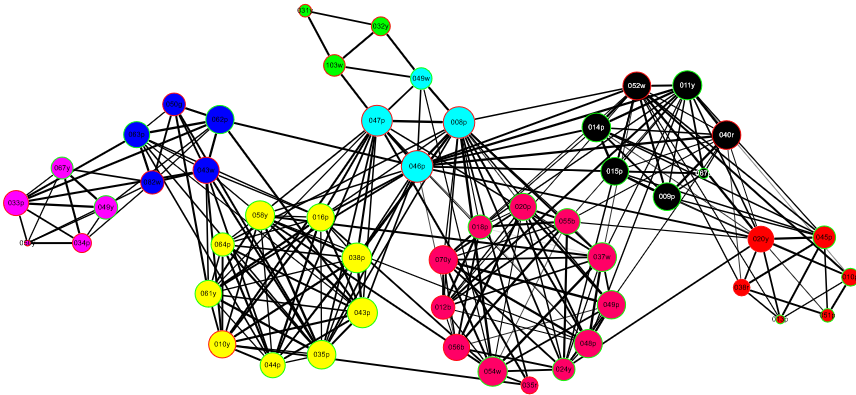
\includegraphics[width=\linewidth]{bace-flow.PNG}
\caption{Graph of the interactions of the badgers.  Node color represents the badgers social group defined by sett, node size represents between group flow-betweenness, edge width represents edge betweenness.} % caption
\label{bace} % add a label to reference it
\end{figure}

\begin{figure}[h]
%\centering % center the figure
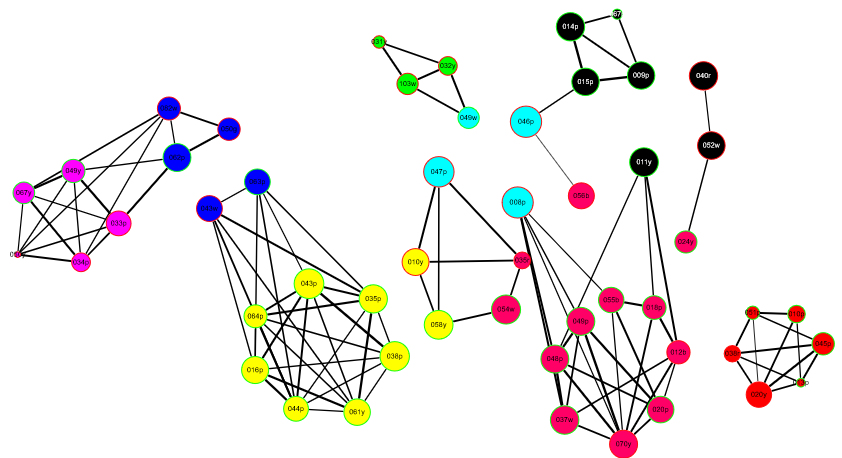
\includegraphics[width=\linewidth]{flow-8.PNG}
\caption{Graph of the interactions of the badgers.  Node color represents the badgers social group defined by sett, node size represents between group flow-betweenness, edge width represents edge betweenness.  Edges were removed vie the Girvan-Newman method to create 8 groups to create 8 groups seen as the 8 connected components seen here.} % caption
\label{flow-8} % add a label to reference it
\end{figure}

\indent The clustering was able to cluster some groups pretty well most of the time.  The yellow, green, and orange group both had a large number of their members in one group.  Some groups did not cluster well at all such as the cyan group and the black group.  There seems to be some sort of correlation between this and the percent of internal nodes (Table \ref{table}).  The yellow and the green groups both had high percent of internal nodes and the cyan and the black group had lower percentages of internal nodes.  


\begin{figure}[h]
%\centering % center the figure
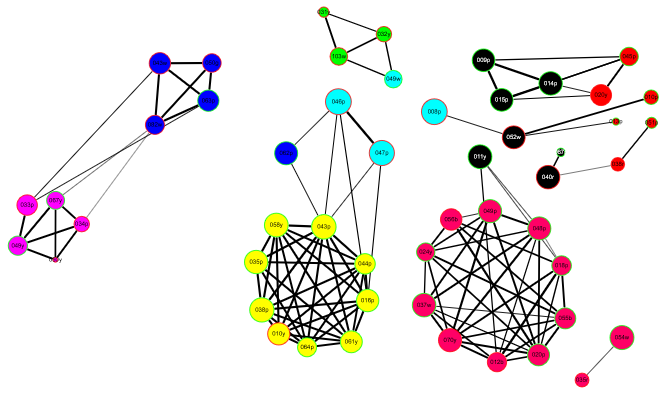
\includegraphics[width=\linewidth]{raw-8.PNG}
\caption{Graph of the interactions of the badgers.  Node color represents the badgers social group defined by sett, node size represents between group flow-betweenness, edge width represents time in contact with.  Edges were removed vie the Girvan-Newman method to create 8 groups to create 8 groups seen as the 8 connected components seen here.} % caption
\label{raw-8} % add a label to reference it
\end{figure}

\indent Ultimately, I think there are some things missing in the time of interaction data that is needed to cluster the badgers into the correct setts.  Webber et. al. (2013) found that badgers with tuberculosis interacted less with their own sett and more with other setts depending on the season.  This could cause badgers to groups into the wrong cluster.  The setts are also spaced differently geographically, this would make it harder or easier for different badgers to interact with any of the setts.  Incorporating this kind of information, possible when calculating edge weights, may make the clustering better for these badgers but it may also make the clustering too specific to this system and not general enough to be useful anywhere else.



\bibliographystyle{plain}
\bibliography{badger}

\end{document}
